\PassOptionsToPackage{numbers,compress}{natbib}
\documentclass{article}
\usepackage[preprint]{neurips_2025}
\makeatletter
\renewcommand{\@noticestring}{}
\makeatother

\usepackage[utf8]{inputenc}
\usepackage[T1]{fontenc}
\usepackage{hyperref}
\usepackage{url}
\usepackage{booktabs}
\usepackage{amsfonts}
\usepackage{nicefrac}
\usepackage{microtype}
\usepackage{xcolor}
\usepackage{graphicx}
\usepackage{multirow}
\usepackage{amsmath}
\usepackage{array}
\usepackage{tikz}
\usepackage{pgfplots}
\pgfplotsset{compat=1.18}

\title{Benchmarking GGUF Quantization for Edge LLM Deployment:\\
A Course Project Study on Pixel 6a with an M4 Comparison}

\author{%
  Kris Dcosta \\
  Halicioglu Data Science Institute \\
  University of California, San Diego \\
  \texttt{kdcosta@ucsd.edu} \\
}

\begin{document}

\maketitle

\begin{abstract}
This project studies a practical edge-AI question: which GGUF quantization levels are most useful when deploying a compact instruction-tuned language model on consumer hardware with tight memory and latency constraints? I built a reproducible benchmarking pipeline and Android application around \texttt{llama.cpp}, then evaluated Llama 3.2 3B Instruct across multiple GGUF variants on a Google Pixel 6a and, as a supplementary comparison, on an Apple M4 Mac with the Metal backend. The Pixel 6a study combines on-device throughput and latency measurements for five core variants, expanded seven-variant quality evaluation on BoolQ and ARC-Easy, and consolidated WikiText-2 perplexity measurements. Three findings are most relevant for deployment. First, the 4-bit family gives the best overall operating region: Q4\_K\_M is the most stable high-throughput option in the main Pixel sweep, while Q4\_K\_S and Q4\_K\_M achieve the strongest downstream quality among the seven-variant evaluation. Second, long-context behavior is highly variant-dependent on mobile hardware: from context length 1024 to 2048, Q3\_K\_M and Q6\_K collapse by more than 50\%, while Q4\_K\_M degrades much more gracefully. Third, quality gains largely plateau beyond the 4-bit boundary: full-corpus WikiText-2 perplexity improves sharply from Q2\_K to the 4-bit variants, then changes only marginally from Q4\_K\_S through Q8\_0. The supplemental M4 comparison shows that quantization ordering depends strongly on hardware backend, reinforcing that deployment guidance cannot be transferred blindly from GPU-oriented results to mobile CPU inference. Power instrumentation was only partially completed and is therefore discussed as preliminary future work rather than a primary result.
\end{abstract}

\section{Introduction}
\label{sec:intro}

Running large language models locally on edge devices is attractive for three reasons: lower latency, improved privacy, and offline availability. In practice, however, deploying even a modest multi-billion-parameter model on a phone is constrained by memory capacity, memory bandwidth, thermal limits, and battery budget. Quantization is therefore not an optional optimization; it is the core mechanism that makes on-device deployment possible.

This course project addresses Topic 4, edge deployment of LLMs. The original proposal focused on building a reproducible local deployment pipeline, measuring prefill and decode throughput, studying context-length scaling, and analyzing the efficiency--accuracy trade-off under multiple quantization levels. Over the course of the project, that scope evolved into a concrete benchmarking study around the GGUF quantization ecosystem used by \texttt{llama.cpp}~\cite{llamacpp}.

The central question is simple but practically important: \emph{which GGUF quantization variant should a practitioner actually deploy on constrained consumer hardware?} Bits per weight alone do not answer this question. A higher-bit model may preserve quality better but run slower, consume more memory, or become unstable at long context lengths. Conversely, an aggressively compressed model may be fast enough for interactive use while sacrificing too much task quality.

This report presents the completed work in a workshop-style paper format. The \textbf{primary platform} is a Google Pixel 6a, where the project implements the intended edge-deployment study. A \textbf{secondary platform}, an Apple M4 Mac using the Metal backend, is included as a comparative system to show how backend and hardware architecture can change the observed quantization ordering. The report emphasizes only the work that is substantiated by the repository artifacts and raw outputs.

The main contributions of the project are:
\begin{enumerate}
  \item A working Android edge-inference application and reproducible benchmark pipeline built around \texttt{llama.cpp}.
  \item A Pixel 6a throughput study across five quantization variants and four context lengths, showing large variant-dependent long-context slowdowns.
  \item A seven-variant quality study using BoolQ, ARC-Easy, and consolidated WikiText-2 perplexity, showing that the strongest deployment region lies in the 4-bit family.
  \item A supplementary seven-variant M4 Metal comparison demonstrating that quantization behavior is hardware-dependent and that GPU-oriented intuition does not always transfer to mobile CPU inference.
\end{enumerate}

\section{Project Scope and Implementation}
\label{sec:scope}

The project was designed as an edge-deployment systems study rather than a pure model-compression paper. The intended deliverables in the proposal were: (1) a reproducible deployment pipeline, (2) quantitative comparison across quantization settings, (3) scaling analysis across context lengths, (4) a simple local demo interface, and (5) a final report discussing deployment trade-offs. Those deliverables were substantially completed.

\textbf{Deployment pipeline.} The repository includes scripts for model handling, benchmarking, quality evaluation, and result aggregation. The project uses \texttt{llama.cpp} as the inference engine, GGUF models as the deployment format, and Android/ADB automation for repeated measurements.

\textbf{Android app.} In addition to the command-line benchmark flow, the project includes an Android application with screens for chat, model management, settings, and benchmark execution. This app was useful both as a demonstration artifact and as a way to validate that the deployment stack worked end to end on the target device.

\textbf{Benchmark assets.} The project contains benchmark datasets for BoolQ, ARC-Easy, ARC-Challenge, HellaSwag, MMLU, and TruthfulQA, plus WikiText-2 text files and imatrix calibration files. Not every dataset appears in the final quantitative claims of this report; only the artifacts with verified, usable outputs are included in the main results.

\section{Experimental Setup}
\label{sec:setup}

\subsection{Hardware and Software}

\textbf{Primary edge device: Google Pixel 6a.} The main target platform is a Pixel 6a with Google Tensor G1, 6\,GB LPDDR5 memory, and Android 16. Inference is run through \texttt{llama.cpp} in CPU mode with four threads, reflecting the project's original goal of studying real on-device deployment under resource constraints.

\textbf{Supplementary comparison device: Apple M4 Mac.} A second experiment set was run on an Apple M4 Mac using the Metal backend. This comparison is not the main scope of the project, but it provides useful context about how quantization interacts with a different hardware and software stack.

\textbf{Model family.} The model family used throughout the report is Llama 3.2 3B Instruct~\cite{llama3}. This is a realistic size for local experimentation: large enough to make quantization meaningful, but small enough to be deployable on the target phone.

\subsection{Quantization Variants}

The project uses the GGUF K-quant family implemented by \texttt{llama.cpp}. Table~\ref{tab:variants} summarizes the variants discussed in the report.

\begin{table}[t]
\centering
\caption{GGUF quantization variants used in the study.}
\label{tab:variants}
\small
\begin{tabular}{lrrp{5.4cm}}
\toprule
\textbf{Variant} & \textbf{Bits/weight} & \textbf{Size (GB)} & \textbf{Notes} \\
\midrule
Q2\_K    & 2.6 & 1.3 & Smallest footprint; aggressive compression \\
Q3\_K\_M & 3.4 & 1.6 & Low-memory option; unstable at long context in Pixel sweep \\
Q4\_K\_S & 4.4 & 1.8 & Strong quality-size trade-off in expanded evaluation \\
Q4\_K\_M & 4.8 & 2.0 & Best stable throughput-quality trade-off in the main Pixel sweep \\
Q5\_K\_M & 5.7 & 2.3 & Higher-bit intermediate variant \\
Q6\_K    & 6.6 & 2.7 & Higher fidelity but large long-context slowdown on Pixel \\
Q8\_0    & 8.5 & 3.4 & Highest-memory baseline among the quantized variants \\
\bottomrule
\end{tabular}
\end{table}

\subsection{Metrics and Datasets}

The project used the following measurements:
\begin{itemize}
  \item \textbf{Decode throughput} in tokens per second.
  \item \textbf{Prefill throughput}, time to first token, and end-to-end latency from the benchmark logs.
  \item \textbf{Task quality} on BoolQ and ARC-Easy using 100-question subsets with Wilson confidence intervals.
  \item \textbf{Perplexity} on WikiText-2, consolidated from the project results.
  \item \textbf{Power and energy} as a preliminary measurement target only. Those numbers are not used as a primary claim in this report.
\end{itemize}

The final report relies on four result sources:
\begin{enumerate}
  \item Pixel throughput aggregates from the benchmark summary table.
  \item BoolQ and imatrix BoolQ results from the consolidated quality JSON.
  \item ARC-Easy corrected results from the fixed overnight run.
  \item Consolidated full-corpus WikiText-2 perplexity values and supplementary M4 throughput summaries.
\end{enumerate}

\subsection{Measurement Coverage}

The completed work is uneven across metrics, and this matters for honest reporting.

\textbf{Pixel throughput coverage.} The main on-device throughput sweep has clean, consolidated results for five variants: Q2\_K, Q3\_K\_M, Q4\_K\_M, Q6\_K, and Q8\_0 over context lengths 256, 512, 1024, and 2048. These are the strongest results for analyzing edge-device latency and context scaling.

\textbf{Seven-variant quality coverage.} BoolQ and ARC-Easy results are available for all seven quantization variants, which allows the report to compare Q4\_K\_S and Q5\_K\_M even though those two variants were not rerun through the same consolidated Pixel throughput table.

\textbf{Supplementary M4 throughput coverage.} The M4 comparison includes all seven variants and is used here as a comparative systems perspective.

\section{Results on Pixel 6a}
\label{sec:pixel}

\subsection{Throughput and Context-Length Scaling}

Table~\ref{tab:pixel_tps} and Figure~\ref{fig:pixel_tps} summarize the main Pixel 6a throughput sweep. Several patterns stand out.

First, raw throughput alone does not follow a simple ``more bits is slower'' or ``fewer bits is better'' rule. At context length 1024, Q4\_K\_M reaches 6.22\,tok/s, while Q6\_K reaches only 4.80\,tok/s despite using a higher-bit representation. This is consistent with the project's broader observation that kernel behavior and memory access patterns matter as much as nominal precision.

Second, long-context behavior is strongly variant-dependent. Q3\_K\_M drops from 6.17\,tok/s at context 1024 to 2.76\,tok/s at context 2048, and Q6\_K drops from 4.80\,tok/s to 1.94\,tok/s. By contrast, Q4\_K\_M decreases from 6.22\,tok/s to 5.26\,tok/s over the same range, remaining much more usable for long prompts or long-running conversations.

Third, the best practical deployment region on the phone is not the highest-bit variant. Q8\_0 remains viable, but its 3.4\,GB footprint is much larger than the 4-bit family while offering no decisive edge in the task-quality results shown later.

\begin{table}[t]
\centering
\caption{Pixel 6a decode throughput summary from the consolidated benchmark table. The ``Drop'' column measures degradation from context length 1024 to 2048.}
\label{tab:pixel_tps}
\small
\begin{tabular}{lrrrr}
\toprule
\textbf{Variant} & \textbf{ctx=256} & \textbf{ctx=1024} & \textbf{ctx=2048} & \textbf{Drop} \\
\midrule
Q2\_K    & 5.83 & 5.45 & 4.60 & $-15.6\%$ \\
Q3\_K\_M & 6.01 & 6.17 & 2.76 & $-55.3\%$ \\
Q4\_K\_M & 5.49 & 6.22 & 5.26 & $-15.4\%$ \\
Q6\_K    & 4.97 & 4.80 & 1.94 & $-59.6\%$ \\
Q8\_0    & 5.49 & 5.40 & 4.23 & $-21.7\%$ \\
\bottomrule
\end{tabular}
\end{table}

For the original edge-deployment objective, this table is one of the most useful outputs of the entire project. If the device must support large contexts, Q3\_K\_M and Q6\_K are poor choices despite looking competitive at shorter contexts. If the goal is balanced interactive performance, Q4\_K\_M is the strongest option among the variants included in the main Pixel throughput sweep.

\begin{figure}[t]
\centering
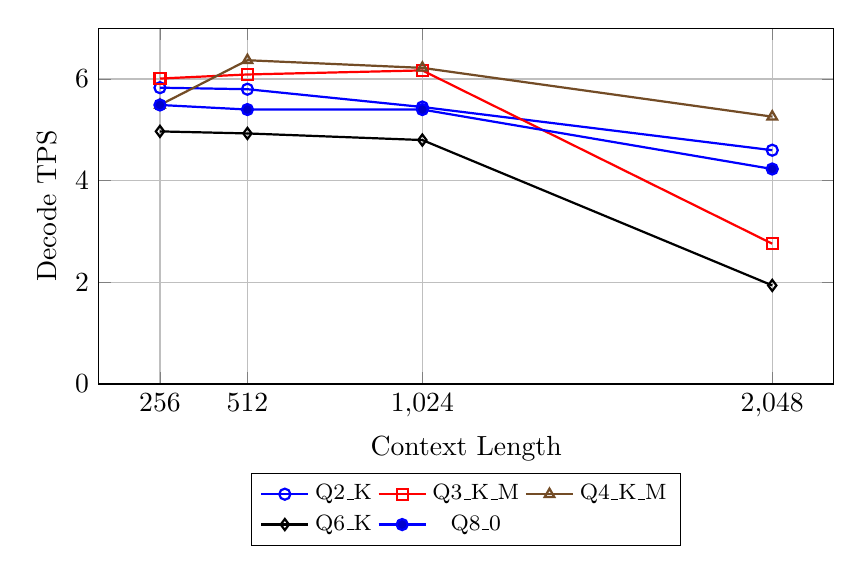
\begin{tikzpicture}
\begin{axis}[
    width=0.9\linewidth,
    height=6.1cm,
    xlabel={Context Length},
    ylabel={Decode TPS},
    ymin=0,
    ymax=7,
    xtick={256,512,1024,2048},
    legend style={font=\footnotesize, at={(0.5,-0.25)}, anchor=north, legend columns=3},
    grid=major,
]
\addplot+[mark=o, thick] coordinates {(256,5.83) (512,5.80) (1024,5.45) (2048,4.60)};
\addplot+[mark=square, thick] coordinates {(256,6.01) (512,6.09) (1024,6.17) (2048,2.76)};
\addplot+[mark=triangle, thick] coordinates {(256,5.49) (512,6.37) (1024,6.22) (2048,5.26)};
\addplot+[mark=diamond, thick] coordinates {(256,4.97) (512,4.93) (1024,4.80) (2048,1.94)};
\addplot+[mark=*, thick] coordinates {(256,5.49) (512,5.40) (1024,5.40) (2048,4.23)};
\legend{Q2\_K,Q3\_K\_M,Q4\_K\_M,Q6\_K,Q8\_0}
\end{axis}
\end{tikzpicture}
\caption{Pixel 6a decode throughput across context lengths for the five variants included in the consolidated on-device throughput sweep. Q3\_K\_M and Q6\_K exhibit the strongest long-context collapse, while Q4\_K\_M remains comparatively stable.}
\label{fig:pixel_tps}
\end{figure}

\subsection{Quality Trade-offs Across Seven Variants}

The expanded seven-variant quality study paints a clearer picture of where quality stabilizes. Table~\ref{tab:quality}, Figure~\ref{fig:quality_scores}, and Figure~\ref{fig:ppl_curve} combine BoolQ, ARC-Easy, and the consolidated WikiText-2 perplexity values.

Three observations are important.

\textbf{1. The 4-bit family is the strongest deployment region.} Q4\_K\_S achieves the highest BoolQ score in the seven-variant quality study at 74\%, while Q4\_K\_M achieves the highest ARC-Easy score at 82\%. Both variants sit near the point where the perplexity curve flattens.

\textbf{2. Perplexity improves sharply before 4 bits, then plateaus.} The change from Q2\_K to Q3\_K\_M is large (13.29 to 11.08), and the change from Q3\_K\_M to Q4\_K\_S is still meaningful (11.08 to 10.70). Above that point, the gap is very small: Q4\_K\_S, Q4\_K\_M, Q5\_K\_M, Q6\_K, and Q8\_0 all fall in a narrow band between 10.58 and 10.71.

\textbf{3. Higher-bit variants are not automatically better on downstream tasks.} Q6\_K and Q8\_0 do not dominate the 4-bit family on BoolQ or ARC-Easy. This is exactly the kind of practical result that matters for edge deployment: once a compact variant crosses the quality threshold needed by the task, extra bits may add memory cost without improving end-user utility.

\begin{table}[t]
\centering
\caption{Seven-variant quality summary on Pixel 6a. BoolQ and ARC-Easy are 100-question evaluations with Wilson 95\% confidence intervals. WikiText-2 perplexity values are consolidated project results.}
\label{tab:quality}
\small
\begin{tabular}{lrrr}
\toprule
\textbf{Variant} & \textbf{BoolQ} & \textbf{ARC-Easy} & \textbf{WikiText-2 PPL} \\
\midrule
Q2\_K    & 69\% $\pm$ 8.9\% & 76\% $\pm$ 8.3\% & 13.29 $\pm$ 0.10 \\
Q3\_K\_M & 69\% $\pm$ 8.9\% & 78\% $\pm$ 8.0\% & 11.08 $\pm$ 0.08 \\
Q4\_K\_S & \textbf{74\% $\pm$ 8.5\%} & 81\% $\pm$ 7.6\% & 10.70 $\pm$ 0.08 \\
Q4\_K\_M & 72\% $\pm$ 8.7\% & \textbf{82\% $\pm$ 7.5\%} & 10.71 $\pm$ 0.08 \\
Q5\_K\_M & 67\% $\pm$ 9.1\% & 81\% $\pm$ 7.6\% & 10.62 $\pm$ 0.08 \\
Q6\_K    & 65\% $\pm$ 9.2\% & 79\% $\pm$ 7.9\% & 10.58 $\pm$ 0.08 \\
Q8\_0    & 68\% $\pm$ 9.0\% & 80\% $\pm$ 7.8\% & 10.59 $\pm$ 0.08 \\
\bottomrule
\end{tabular}
\end{table}

\begin{figure}[t]
\centering
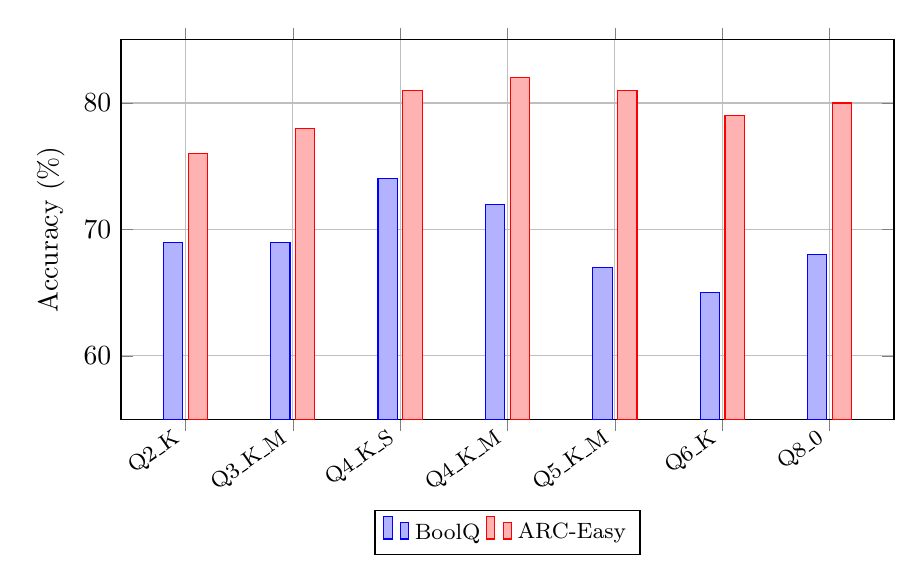
\begin{tikzpicture}
\begin{axis}[
    ybar,
    bar width=7pt,
    width=0.94\linewidth,
    height=6.4cm,
    ymin=55,
    ymax=85,
    ylabel={Accuracy (\%)},
    symbolic x coords={Q2\_K,Q3\_K\_M,Q4\_K\_S,Q4\_K\_M,Q5\_K\_M,Q6\_K,Q8\_0},
    xtick=data,
    x tick label style={rotate=35, anchor=east, font=\footnotesize},
    legend style={font=\footnotesize, at={(0.5,-0.24)}, anchor=north, legend columns=2},
    grid=major,
]
\addplot coordinates {(Q2\_K,69) (Q3\_K\_M,69) (Q4\_K\_S,74) (Q4\_K\_M,72) (Q5\_K\_M,67) (Q6\_K,65) (Q8\_0,68)};
\addplot coordinates {(Q2\_K,76) (Q3\_K\_M,78) (Q4\_K\_S,81) (Q4\_K\_M,82) (Q5\_K\_M,81) (Q6\_K,79) (Q8\_0,80)};
\legend{BoolQ,ARC-Easy}
\end{axis}
\end{tikzpicture}
\caption{Seven-variant downstream task quality on Pixel 6a. The 4-bit family is the strongest overall operating region: Q4\_K\_S leads BoolQ and Q4\_K\_M leads ARC-Easy.}
\label{fig:quality_scores}
\end{figure}

\begin{figure}[t]
\centering
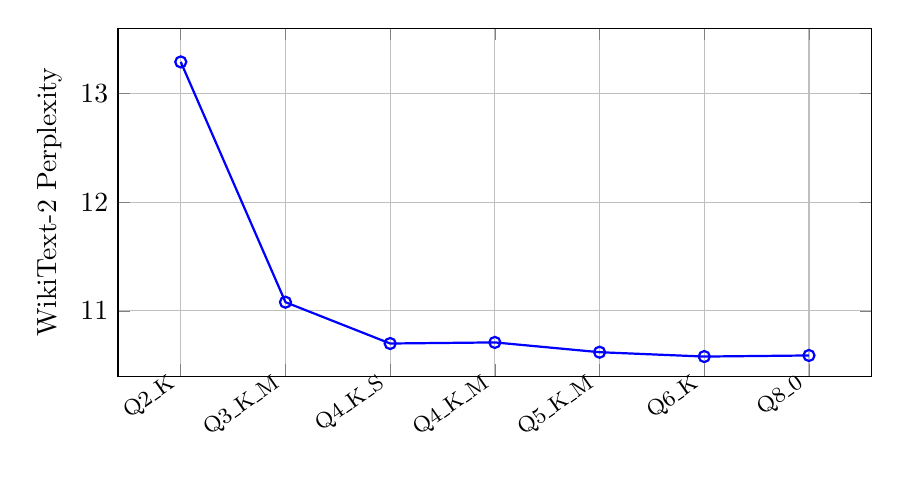
\begin{tikzpicture}
\begin{axis}[
    width=0.92\linewidth,
    height=6cm,
    ylabel={WikiText-2 Perplexity},
    ymin=10.4,
    ymax=13.6,
    symbolic x coords={Q2\_K,Q3\_K\_M,Q4\_K\_S,Q4\_K\_M,Q5\_K\_M,Q6\_K,Q8\_0},
    xtick=data,
    x tick label style={rotate=35, anchor=east, font=\footnotesize},
    grid=major,
]
\addplot+[mark=o, thick] coordinates {(Q2\_K,13.29) (Q3\_K\_M,11.08) (Q4\_K\_S,10.70) (Q4\_K\_M,10.71) (Q5\_K\_M,10.62) (Q6\_K,10.58) (Q8\_0,10.59)};
\end{axis}
\end{tikzpicture}
\caption{Consolidated full-corpus WikiText-2 perplexity values. The major quality improvement occurs before the 4-bit boundary; beyond Q4\_K\_S the curve is nearly flat.}
\label{fig:ppl_curve}
\end{figure}

\subsection{A Note on imatrix Calibration}

The repository also contains an imatrix-calibrated BoolQ evaluation. Those results are interesting but mixed. Q4\_K\_S-imatrix reaches 75\% on BoolQ, slightly above the non-imatrix Q4\_K\_S run, while other calibrated variants do not show a uniform gain. Because the calibration study was narrower than the main benchmark suite, I treat it as a supporting observation rather than a headline result: calibration can help, but its effects were not consistently monotonic across all variants in the available runs.

\section{Supplementary Comparison on Apple M4}
\label{sec:m4}

The M4 experiments provide a useful comparison because they expose the same quantized model family to a very different backend. Table~\ref{tab:m4} and Figure~\ref{fig:m4_tps} report the consolidated decode throughput summary at context length 2048.

\begin{table}[t]
\centering
\caption{Supplementary M4 Metal decode throughput at context length 2048 from the consolidated summary tables.}
\label{tab:m4}
\small
\begin{tabular}{lr}
\toprule
\textbf{Variant} & \textbf{Decode TPS} \\
\midrule
Q2\_K    & 30.42 \\
Q3\_K\_M & 26.15 \\
Q4\_K\_S & 27.01 \\
Q4\_K\_M & \textbf{30.62} \\
Q5\_K\_M & 20.25 \\
Q6\_K    & 21.43 \\
Q8\_0    & 17.51 \\
\bottomrule
\end{tabular}
\end{table}

\begin{figure}[t]
\centering
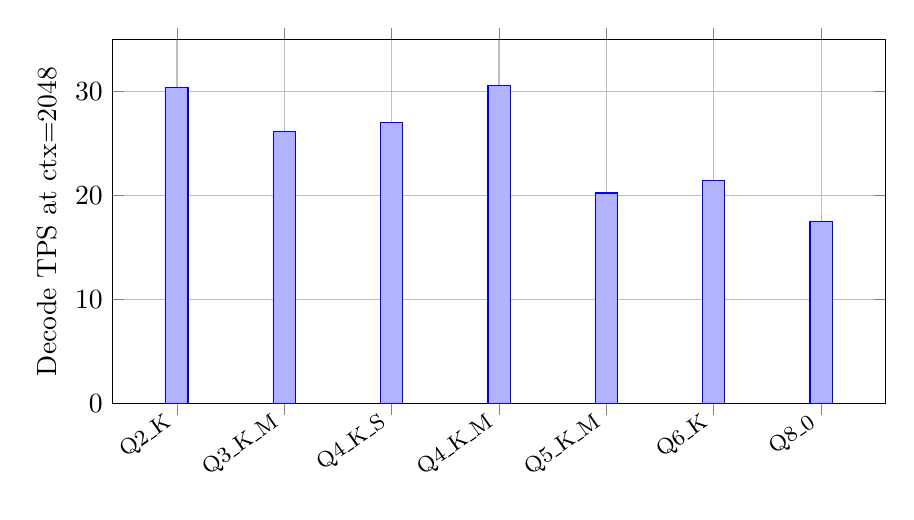
\begin{tikzpicture}
\begin{axis}[
    ybar,
    bar width=8pt,
    width=0.94\linewidth,
    height=6.2cm,
    ymin=0,
    ymax=35,
    ylabel={Decode TPS at ctx=2048},
    symbolic x coords={Q2\_K,Q3\_K\_M,Q4\_K\_S,Q4\_K\_M,Q5\_K\_M,Q6\_K,Q8\_0},
    xtick=data,
    x tick label style={rotate=35, anchor=east, font=\footnotesize},
    grid=major,
]
\addplot coordinates {(Q2\_K,30.42) (Q3\_K\_M,26.15) (Q4\_K\_S,27.01) (Q4\_K\_M,30.62) (Q5\_K\_M,20.25) (Q6\_K,21.43) (Q8\_0,17.51)};
\end{axis}
\end{tikzpicture}
\caption{Supplementary Apple M4 Metal decode throughput at context length 2048. The ordering differs from the Pixel edge-device results, reinforcing that quantization choices are backend-dependent.}
\label{fig:m4_tps}
\end{figure}

The main value of this table is not the ranking itself, but the contrast with the Pixel results. On the phone, long-context performance makes Q3\_K\_M and Q6\_K particularly unattractive. On the M4 summary, Q4\_K\_M and Q2\_K are the strongest long-context performers, and the ordering differs from what one would infer from the quality table alone. This supports a broader lesson: quantization decisions are hardware-dependent. A recommendation derived from one backend should not be assumed to transfer unchanged to another.

The repository also contains a finer-grained M4 context sweep focused on the KV-cache behavior of selected variants. In the broader project narrative, those measurements were used to study long-context regime changes on Metal. For the purposes of this course report, the important point is simpler: the M4 comparison reinforces the systems perspective of the project by showing that edge-deployment guidance must be tied to actual hardware measurements rather than to bits-per-weight heuristics.

\section{Discussion}
\label{sec:discussion}

The project set out to study whether a compact LLM could be deployed meaningfully on a constrained edge device and which quantization settings make that deployment practical. The completed results support three deployment conclusions.

\textbf{The best operating region is around 4 bits.} Across the verified quality results, the 4-bit family consistently gives the most attractive trade-off. Q4\_K\_S and Q4\_K\_M preserve most of the quality gains that appear after leaving the low-bit regime, yet avoid the memory overhead of Q6\_K and Q8\_0. On the phone, Q4\_K\_M is also the most stable long-context option among the variants covered in the main throughput sweep.

\textbf{Long-context behavior matters as much as average throughput.} If one looked only at shorter contexts, Q3\_K\_M could appear competitive. At context length 2048, that impression collapses. This is a practically important lesson for edge deployment: a model that looks acceptable in a short prompt benchmark may become unusable in realistic interactive settings with longer histories.

\textbf{Edge benchmarking should be end-to-end, not just model-centric.} A major part of the value of this project is that it did not stop at model files or synthetic complexity estimates. The work includes application integration, repeated on-device measurements, context scaling, and downstream task checks. That end-to-end approach is necessary if the goal is to recommend an actual deployment configuration rather than just compare abstract quantization formats.

In addition, the M4 comparison clarified a methodological point that will be useful beyond this specific project. Hardware backend differences can change which quantization variants look best. For that reason, edge deployment papers and engineering reports should be explicit about the device, backend, context length, and evaluation task when making practical recommendations.

\section{Limitations and Future Work}
\label{sec:limitations}

This project has several limitations that should be stated clearly.

\textbf{Single primary edge device.} The core edge-deployment study was conducted on a single phone model, the Pixel 6a. That is appropriate for a course project and sufficient to support device-specific conclusions, but it does not justify claims about all mobile hardware.

\textbf{Uneven coverage across metrics.} The cleanest throughput sweep on Pixel covers five variants, while the cleanest quality study covers seven. This means the report can compare all seven variants on quality, but not every variant appears in the same consolidated Pixel throughput table.

\textbf{Preliminary power instrumentation.} Power measurement was part of the intended project scope only ``if feasible,'' and in practice it turned out to be the least mature measurement stream. The repository includes instrumentation scripts and partial outputs, but I do not treat those results as strong enough for a primary quantitative claim. Completing and validating the power study is a natural next step.

\textbf{Consolidated perplexity results.} The WikiText-2 perplexity values used in the report were consolidated into the project summary. They are useful for identifying the quality plateau beyond 4 bits, but a future revision should connect every reported value directly to a dedicated raw-result artifact in the same level of detail as the throughput and task-quality tables.

\textbf{Additional datasets remain out of scope for the final report claims.} The repository contains assets and partial work for ARC-Challenge, HellaSwag, MMLU, and TruthfulQA. Those are useful foundations for follow-up work, but they are not needed to support the main edge-deployment conclusions presented here.

Future work should therefore focus on three directions: (1) complete and clean the partial power measurements, (2) extend the main on-device throughput sweep to the newer seven-variant set so that throughput and quality can be compared on exactly the same coverage, and (3) test whether the 4-bit ``best operating region'' result generalizes to additional phones and model families.

\section{Conclusion}
\label{sec:conclusion}

This project demonstrates that benchmarking quantization for edge LLM deployment is not just a model-compression exercise; it is a systems problem. By building an Android deployment stack, running repeated measurements on a Pixel 6a, and comparing the results with a supplementary M4 Metal study, the project shows that practical deployment decisions depend on the interaction among quantization format, context length, hardware backend, and task quality.

The clearest conclusion is that the 4-bit family is the most useful region for deployment on the studied hardware. Q4\_K\_M emerged as the best stable throughput option in the main Pixel sweep, while Q4\_K\_S and Q4\_K\_M provided the strongest quality results among the seven-variant evaluation. At the same time, the project shows why short-context throughput alone is not enough: Q3\_K\_M and Q6\_K degrade severely at long context on the phone, making them poor practical choices for real interactive workloads.

More broadly, the project met its original edge-deployment goals. It produced a working local application, a reproducible benchmarking pipeline, a quantitative comparison across quantization settings, and a clear set of deployment lessons grounded in completed experiments. That combination of implementation and analysis is the main outcome of the work.

\bibliographystyle{plain}
\begin{thebibliography}{10}

\bibitem{llamacpp}
Georgi Gerganov et al.
\newblock llama.cpp: LLM inference in C/C++.
\newblock \url{https://github.com/ggerganov/llama.cpp}, 2023.

\bibitem{llama3}
Meta AI.
\newblock The Llama 3 Herd of Models.
\newblock \emph{arXiv preprint arXiv:2407.21783}, 2024.

\bibitem{gptq}
Elias Frantar, Saleh Ashkboos, Torsten Hoefler, and Dan Alistarh.
\newblock GPTQ: Accurate Post-Training Quantization for Generative Pre-Trained Transformers.
\newblock In \emph{International Conference on Learning Representations}, 2023.

\bibitem{awq}
Ji Lin, Jiaming Tang, Haotian Tang, Shang Yang, Wei-Ming Chen, Guangxuan Xiao,
Xingyu Dang, Chuang Gan, and Song Han.
\newblock AWQ: Activation-Aware Weight Quantization for On-Device LLM Compression and Acceleration.
\newblock In \emph{Proceedings of Machine Learning and Systems}, 2024.

\bibitem{mobileaibench}
Rithesh Murthy, Liangwei Yang, Juntao Tan, et al.
\newblock MobileAIBench: Benchmarking LLMs and LMMs for On-Device Use Cases.
\newblock \emph{arXiv preprint arXiv:2406.10290}, 2024.

\bibitem{llminference}
Zhihang Yuan, Yuzhang Shang, Yang Zhou, Zhen Dong, et al.
\newblock LLM Inference Unveiled: Survey and Roofline Model Insights.
\newblock \emph{arXiv preprint arXiv:2402.16363}, 2024.

\bibitem{boolq}
Christopher Clark, Kenton Lee, Ming-Wei Chang, Tom Kwiatkowski,
Michael Collins, and Kristina Toutanova.
\newblock BoolQ: Exploring the Surprising Difficulty of Natural Yes/No Questions.
\newblock In \emph{Proceedings of NAACL-HLT}, 2019.

\bibitem{arc}
Peter Clark, Isaac Cowhey, Oren Etzioni, Tushar Khot, Ashish Sabharwal,
Carissa Schoenick, and Oyvind Tafjord.
\newblock Think You Have Solved Question Answering? Try ARC, the AI2 Reasoning Challenge.
\newblock \emph{arXiv preprint arXiv:1803.05457}, 2018.

\bibitem{wikitext2}
Stephen Merity, Caiming Xiong, James Bradbury, and Richard Socher.
\newblock Pointer Sentinel Mixture Models.
\newblock In \emph{International Conference on Learning Representations}, 2017.

\bibitem{applem4}
Apple Inc.
\newblock Apple introduces M4 chip.
\newblock \url{https://www.apple.com/newsroom/2024/05/apple-introduces-m4-chip/}, 2024.

\end{thebibliography}

\end{document}
